% !TEX root = develop_pairs_short.tex
\section{Preliminary Evaluation}
To evaluate our approach we analyzed collaboration and build data in the IBM Rational Team Concert\texttrademark\ (RTC) development team.
RTC is a product that integrates source code management, agile planning, and issue management into a single server/client application that the team itself uses for development.
RTC allows developers to link changes they made directly to work items, thus establishing within their repository traceable links between builds and work items through the changes they made.
The repository spans three months in which the team started 326 builds, 99 of which failed and 227 that were successful. 
The team consists of more than 100 developers distributed across seven major sites in Europe, Asia, and North America. Due to the team's geographical distribution and agile development process the team's  communication is largely found in the online repository in the form of comments related to work items. 


In RTC we conceptualize a \emph{technical pair} as two developers that modified the same file in a build.
Similarly, two developers are in a \emph{socio-technical pair} if they modified the same file in a build \emph{and} commented on a work item that was linked to the build in which they changed the same file.

\begin{table}[t]
\centering
%\subtable[Twenty most frequent \emph{technical pairs} that are failure-related.]{
\begin{tabular}{@{\hspace{.2cm}}ccc@{\hspace{.75cm}}c@{\hspace{.2cm}}}
\toprule
Pair & \#successful & \#failed & $p_x$\\
\midrule
%Cody-Daisy&  0 & 12 & 1.0000 \\
%Adam-Ina & 0 & \phantom{1}8 & 1.0000 \\
%Adam-Kim& 0 & \phantom{1}8 & 1.0000 \\
%Adam-Nina & 0 & \phantom{1}6 & 1.0000 \\
%Fred-Gina& 0 & \phantom{1}6 & 1.0000 \\
%Gina-Oliver & 0 & \phantom{1}6 & 1.0000 \\
%Adam-Daisy& 1 & 14 & 0.9720\\%67 \\
%Bart-Daisy& 1 & \phantom{1}9 & 0.9572\\%127 \\
%Adam-Lisa& 1 & \phantom{1}8 & 0.9521\\%204 \\
%Bart-Eve & 2 & 11 & 0.9318\\%403 \\
%\textbf{Adam}-\textbf{Bart}& \textbf{3} & \textbf{13} & \textbf{0.9150}\\%485 \\
%Bart-Cody & 3 & 13 & 0.9150\\%485 \\
%Adam-Eve & 4 & 16 & 0.9086\\%162 \\
%Daisy-Ina & 3 & 12 & 0.9086\\%162 \\
%Cody-Fred& 3 & 10 & 0.8923\\%077 \\
%Bart-Herb & 3 & 10 & 0.8923\\%077 \\
%Cody-Eve & 5 & 15 & 0.8817\\%568 \\
%Adam-Jim & 4 & 11 & 0.8723\\%792 \\
%Herb-Paul & 5 & 12 & 0.8564\\%397 \\
%Mike-Rob& 6 & 13 & 0.8434\\%004\\
%Adam-Fred & 6 & 13 & 0.8434\\%004\\
%
%User11137, User4105 & 0 & 12 & 1.0000 \\
%User2943, User13877 & 0 & 8 & 1.0000 \\
%User7438, User2943 & 0 & 8 & 1.0000 \\
%User2943, User2810 & 0 & 6 & 1.0000 \\
%User8645, User1976 & 0 & 6 & 1.0000 \\
%User8645, User2267 & 0 & 6 & 1.0000 \\
%User11137, User2943 & 1 & 14 & 0.9675\\%908 \\
%User11137, User3493 & 1 & 9 & 0.9504\\%773 \\
%User6012, User2943 & 1 & 8 & 0.9446\\%298 \\
%User3493, User2435 & 2 & 11 & 0.9214\\%387 \\
%User3493, User2943 & 3 & 13 & 0.9023\\%53 \\
%User3493, User4105 & 3 & 13 & 0.9023\\%53 \\
%User2943, User2435 & 4 & 16 & 0.8950\\%695 \\
%User11137, User13877 & 3 & 12 & 0.8950\\%695 \\
%User1976, User4105 & 3 & 10 & 0.8766\\%716 \\
%User3493, User6339 & 3 & 10 & 0.8766\\%716 \\
%User4105, User2435 & 5 & 15 & 0.8648\\%208 \\
%User2943, User9017 & 4 & 11 & 0.8543\\%22 \\
%User6339, User13875 & 5 & 12 & 0.8365\\%498 \\
%User10979, User3385 & 6 & 13 & 0.8220\\%793\\
%User2943, User1976 & 6 & 13 & 0.8220\\%793 \\
%
(Cody, Daisy)	&	0&	12&	1		\\ %user11137.user4105.T
(Adam, Daisy)	&	1&	14&	0.9697	\\ %user11137.user2943.T
(Bart, Eve)	&	2&	11&	0.9265	\\ %user3493.user2435.T
(Adam, Bart)	&	3&	13&	0.9085	\\ %user3493.user2943.T
(Bart, Cody)	&	3&	13&	0.9085	\\ %user3493.user4105.T
(Adam, Eve)	&	4&	16&	0.9016	\\ %user2943.user2435.T
(Daisy, Ina)	&	3&	12&	0.9016	\\ %user11137.user13877.T
(Cody, Fred)	&	3&	10&	0.8843	\\ %user1976.user4105.T
(Bart, Herb)	&	3&	10&	0.8843	\\ %user3493.user6339.T
(Cody, Eve)	&	5&	15&	0.8730	\\ %user4105.user2435.T
(Adam, Jim)	&	4&	11&	0.8631	\\ %user2943.user9017.T
(Herb, Paul)	&	5&	12&	0.8462	\\ %user6339.user13875.T
(Cody, Fred)	&	5&	11&	0.8345	\\ %user11137.user1976.T
(Mike, Rob)	&	6&	13&	0.8324	\\ %user10979.user3385.T
(Adam, Fred)	&	6&	13&	0.8324	\\ %user2943.user1976.T
(Daisy, Fred)	&	8&	13&	0.7884	\\ %user3493.user1976.T
(Gill, Eve)		&	7&	10&	0.7661	\\ %user1264.user2435.T
(Daisy, Ina)	&	7&	10&	0.7661	\\ %user3493.user13873.T
(Fred, Ina)	&	8&	10&	0.7413	\\ %user1976.user13877.T
(Herb, Eve)	&	8&	10&	0.7413	\\ %user6339.user2435.T
\bottomrule
\end{tabular}
%\caption{Twenty \emph{technical pairs} that are failure-related and affect the most builds.}
%\label{tab:badtechpairs}
%}\hspace{1.3cm}
%\end{table}
%
%\subtable[The twenty corresponding \emph{socio-technical pairs}, which are not statistically related to failed builds.]{
%\begin{tabular}{@{\hspace{.2cm}}ccc@{\hspace{.75cm}}c@{\hspace{.2cm}}}
%\toprule
%Pair & \#successful & \#failed & $p_x$ \\
%\midrule
%(Cody, Daisy)	&	---&	---&	---\\
%(Adam, Daisy)	&	---&	---&	---\\
%(Bart, Eve)	&	1&	4&	0.9016\\
%(Adam, Bart)	&	---&	---&	---\\
%(Bart, Cody)	&	---&	---&	---\\
%(Adam, Eve)	&	---&	---&	---\\
%(Daisy, Ina)	&	---&	---&	---\\
%(Cody, Fred)	&	1&	0&	0\\
%(Bart, Herb)	&	1&	2&	0.8209\\
%(Cody, Eve)	&	0&	3&	1\\
%(Adam, Jim)	&	0&	1&	1\\
%(Herb, Paul)	&	1&	0&	0\\
%(Cody, Fred)	&	---&	---&	---\\
%(Mike, Rob)	&	---&	---&	---\\
%(Adam, Fred)	&	---&	---&	---\\
%(Daisy, Fred)	&	---&	---&	---\\
%(Gill, Eve)		&	---&	---&	---\\
%(Daisy, Ina)	&	1&	0&	0\\
%(Fred, Ina)	&	0&	2&	1\\
%(Herb, Eve)	&	---&	---&	---\\
%\bottomrule
%\end{tabular}
%%\caption{Twenty \emph{technical pairs} that are failure-related and affect the most builds.}
%\label{tab:stechpairs}
%}
\caption{The top 20 statistically failure related technical pairs.}
\label{tab:pairs}
\vspace{-20pt}
\end{table}

\emph{Preliminary Results.}
Using our approach we analyzed all existing builds in the project and were able to identify a ranked list of 120 developer pairs that should communicate in order to increase the likelihood of the upcoming build to succeed. 

We used the approach as follows: From the total of 2872 developer pairs, we found 961 technical pairs (set $T$) (step 1).
Of these 961 technical pairs we found 120 harmful pairs (set $H$) that were statistically related to build failure (step 2). See Table~\ref{tab:pairs} for the top twenty  pairs.

Next, for all pairs in set $H$, we examined their corresponding \emph{socio-technical pairs} (step 3). Because this set ($H_f$) was empty in our data we did not have to remove any pairs from $H$. 
In step 4 we identified that none of the 120 technical pairs in $R$ had an existing corresponding socio-technical pair related to build success nor failure. Thus $R_1$ was empty and $R=R_2$. 

%Thus, step 4 yields $R_1$ containing no recommendations and $R_2$ containing 120 recommendations in the form of technical pairs.

In step 5 we ranked the recommendations in $R$
by the coefficient $p_{x}$ as shown in Table~\ref{tab:pairs}. This coefficient indicates the strength of
relationship between the developer pair and build failure. For instance, the
developer pair (Adam, Bart), appears in 13 failed builds and in 3
successful builds. This means that pair$_{failed}$ = 13 and pair$_{success}$ = 3
with total$_{failed}$= 99 and total$_{success}$= 227 result in $p_x$= 0.9016.


\begin{figure}[t]
\vspace{-29pt}
\centering
%\subfigure[Evaluation results from the Support Vector Machine.] {
%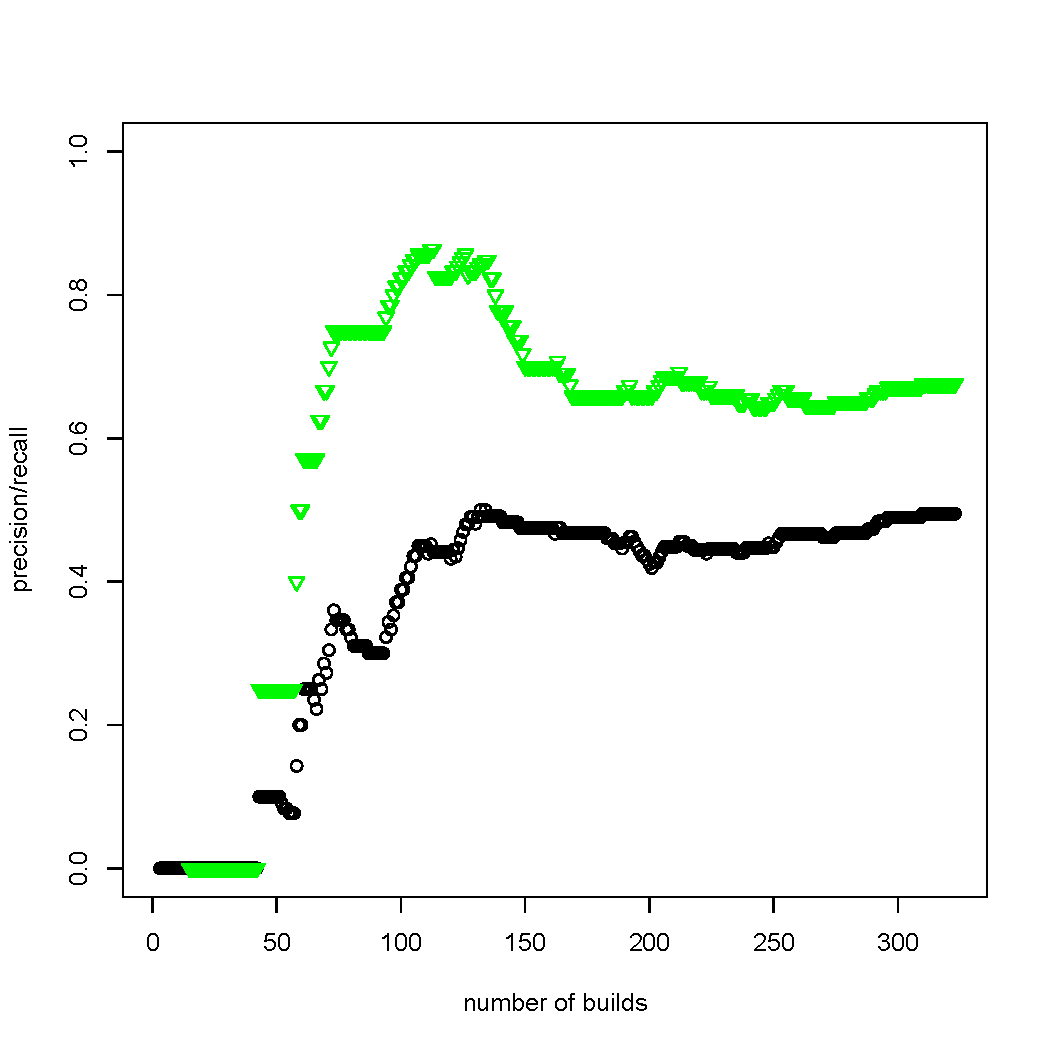
\includegraphics[width=\columnwidth]{precission-recall}
%\label{fig:prediction-svm}
%}
%\subfigure[Evaluation results from the Logistic Regression.] {
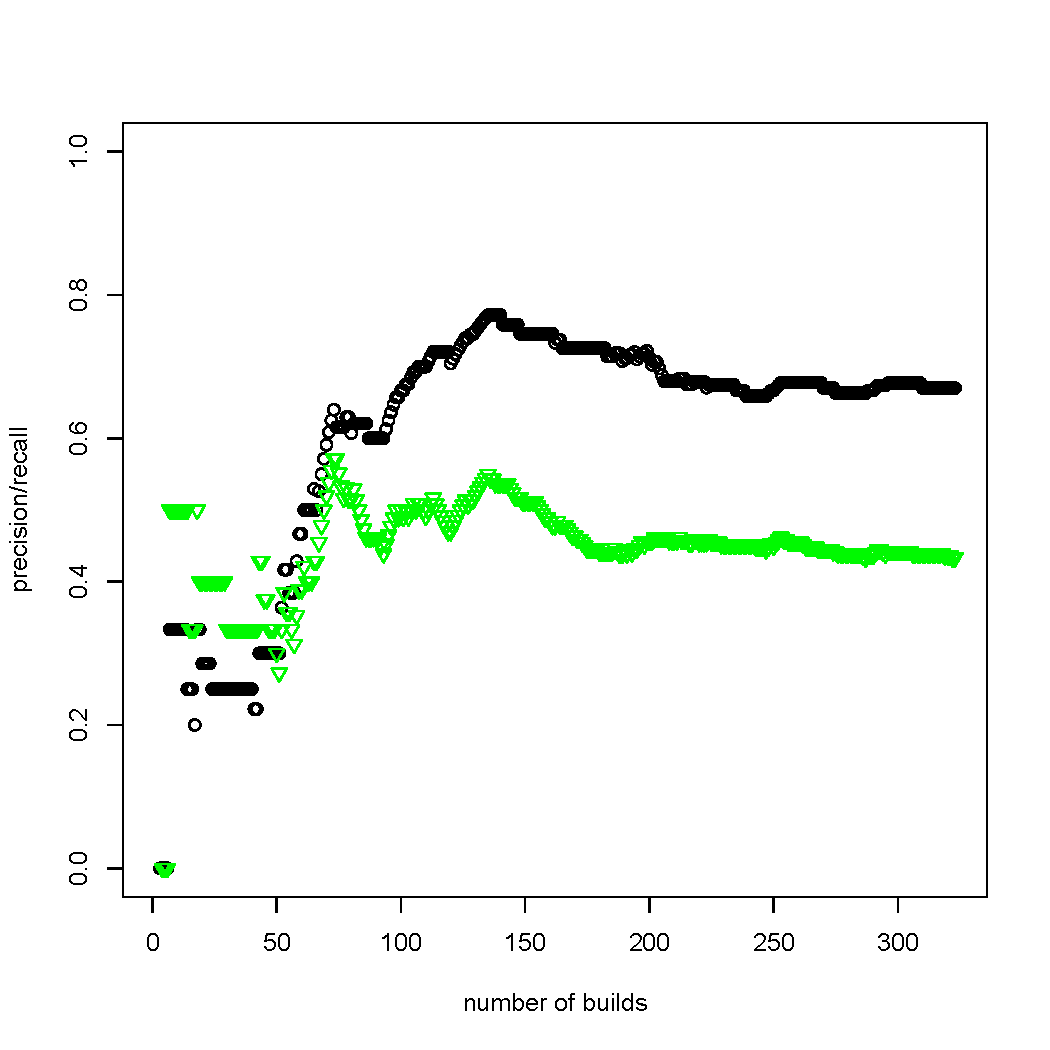
\includegraphics[width=\columnwidth]{precision-recall-logreg}
%\label{fig:prediction-logreg}
%}
\vspace{-25pt}
\caption{Precision (green) and recall (black) of the logistic regression.}
\label{fig:prediction}
\vspace{-10pt}
\end{figure}

To further validate our recommendations, we used the approach to generate a list of technical pairs for each of the 326 builds in our data. For any given build N we used the technical pairs as recommended by our approach from all the previous builds to build a logistical regression model predicting the outcome of build N. 
Applying this method to all builds yields Figure~\ref{fig:prediction} which shows the recall (black) and precision (green) values for the a logistical regression model used for prediction.
The recall and precision are cumulative at each point, including the prediction results obtained for the previous builds.
The logistical regression ended with a precision and recall value of $.43$ (median: $.45$) and $.67$ (median: $.67$) respectively, thus outperforming a random guess based on the ratio between failed and successful builds.
This further suggests that the recommendations that our approach identifies might prevent build failure. 

%WHAT DO THOSE NUMBERS FOR THE PREDICTION MEAN

In seeking explanations for the lack of communication in the RTC technical pairs found by our analysis, we were able to identify that most of these technical pairs consisted of developers belonging to
different teams. This confirms Naggappan et al.~\cite{nagappan:icse:2008}'s result that organizational distance predicts failures. Although the RTC team strongly emphasizes communication
regardless of team boundaries, it still seems that organizational distance had
an influence on its communication behaviour.

\emph{Threats to Validity.}
\label{sec:threats}
First, we performed our preliminary evaluation on one set of data, the Rational Team Concert\texttrademark\
repository, limiting the generalizability of our findings.
However, since the three months  we studied were directly before a major release of the project, 
we believe that this dataset is representative of a period in which lack of coordination (gaps) have the biggest impact on builds. Secondly, we assumed that every developer commenting on, or subscribed to, a work item reads all comments of that work item. 
By manual inspection of a selected number of work items, we found that developers who commented on a work item were aware of the other comments, confirming our assumption.

%Thirdly, Socio-technical dependencies may suffer from the combination of social and technical dependencies. 
%Social dependencies might not be related to the code changes the technical dependency was inferred from.
%Since the changes we used are directly linked to work item discussion we are confident that the vast majority of matches are appropriate.